% Created 2016-12-02 Fri 10:45
\documentclass[bigger]{beamer}
\usepackage[utf8]{inputenc}
\usepackage[T1]{fontenc}
\usepackage{fixltx2e}
\usepackage{graphicx}
\usepackage{grffile}
\usepackage{longtable}
\usepackage{wrapfig}
\usepackage{rotating}
\usepackage[normalem]{ulem}
\usepackage{amsmath}
\usepackage{textcomp}
\usepackage{amssymb}
\usepackage{capt-of}
\usepackage{hyperref}
\mode<beamer>{\useinnertheme{rounded}\usecolortheme{rose}\usecolortheme{dolphin}\setbeamertemplate{navigation symbols}{}\setbeamertemplate{footline}[frame number]{}}
\mode<beamer>{\usepackage{amsmath,amsthm,amssymb,mathtools,tikz,multirow}\usepackage{ae,aecompl}}
\let\oldframe\frame\renewcommand\frame[1][allowframebreaks]{\oldframe[#1]}
\setbeamertemplate{frametitle continuation}[from second]
\usetheme{default}
\author{Ole Jann and Christoph Schottmüller}
\date{}
\title{An informational theory of privacy}
\hypersetup{
 pdfauthor={Ole Jann and Christoph Schottmüller},
 pdftitle={An informational theory of privacy},
 pdfkeywords={},
 pdfsubject={},
 pdfcreator={Emacs 24.5.1 (Org mode 8.3.3)}, 
 pdflang={English}}
\begin{document}

\maketitle
\begin{frame}{Outline}
\tableofcontents
\end{frame}


\section{Introduction}
\label{sec:orgheadline6}

\begin{frame}[label={sec:orgheadline1}]{What is privacy (in this paper)?}
\begin{itemize}
\item ability to take actions without being observed, and having interactions with others confined to the intended recipients
\item (many other definitions)
\item privacy \(\subset\) asymmetric information
\end{itemize}
\end{frame}

\begin{frame}[label={sec:orgheadline2}]{Privacy is hot topic}
Privacy in news and life: 
\begin{itemize}
\item government mass surveillance
\item business mass surveillance
\begin{itemize}
\item e-business: data as side product of any transaction
\item loyalty cards (AH Bonuskaart)
\end{itemize}
\item voluntary provision of private data (facebook, twitter, mobile phone)
\item micro targeting in election campaigns
\end{itemize}

What is at stake? trade-offs? mechanisms?
\end{frame}




\begin{frame}[label={sec:orgheadline3}]{Economics of privacy: Chicago school (Stigler 80, Posner 81)}
\begin{itemize}
\item privacy = asymmetric information
\item asymmetric information = inefficiency (Akerlof, Mirrlees etc.)
\end{itemize}

\(\Rightarrow\) privacy = inefficiency 
\end{frame}

\begin{frame}[label={sec:orgheadline4}]{Popular debate: "Nothing to hide"}
\begin{itemize}
\item reiterated by Google, facebook, NSA etc.
\begin{itemize}
\item If you have nothing to hide, you do not need privacy.
\item If you have something to hide, you should not do it.
\end{itemize}

\item (similar to Chicago school)
\end{itemize}
\end{frame}


\begin{frame}[label={sec:orgheadline5}]{This paper}
\begin{itemize}
\item our model:
\begin{itemize}
\item information is not perfect (correlation: statistical discrimination literature, Phelps 72, Arrow 73)
\item privacy affects behavior
\end{itemize}
\item main result: privacy can be efficient even when considering \emph{informational effects only} (and we show when)
\item other results:
\begin{itemize}
\item lack of privacy changes behavior in one direction ("chilling effects")
\item effectiveness of privacy intrusion is easily overstated
\item privacy is redistributive (affects different people differently)
\item mandating privacy might be necessary to avoid unraveling
\end{itemize}
\end{itemize}
\end{frame}



\section{Model}
\label{sec:orgheadline10}

\begin{frame}[label={sec:orgheadline7}]{Model: An example}
\begin{itemize}
\item Alice thinks drugs should be legalized and wants to write on her facebook profile about that.
\item She is also looking for a job.
\item employers do not want to hire drug users
\item positive correlation between stand on legalization (\(\theta_i\)) and drug use (\(\tau_i\))
\item Two cases: The employer can see what Alice does online, or not.
\end{itemize}
\end{frame}



\begin{frame}[label={sec:orgheadline8}]{Model I}
\begin{itemize}
\item \(n\) individuals
\item individual \(i\) has type \((\theta_i,\tau_i)\)
\begin{itemize}
\item \(\theta_i\sim\Phi(0,1)\), \(\tau_i\) positively correlated with \(\theta_i\) (formally: distribution of \(\tau_{\text{i}}\) at \(\theta_{\text{i}}\)' fosd distribution at \(\theta_{\text{i}}\)''<\(\theta\)')
\end{itemize}
\end{itemize}
\end{frame}

\begin{frame}[label={sec:orgheadline9}]{Model II}
\begin{enumerate}
\item information aggregation stage:
\begin{itemize}
\item \(i\) observes \((\theta_i,\tau_i)\)
\item \(i\) chooses \(p_i\in\{0,1\}\)
\item policy \(p\in\{0,1\}\) is implemented with probability \(q(m/n)\) where \(m/n\) is fraction of individuals choosing \(p_i=1\)
\item \(q'>0\) and \(q\) point symmetric around 0.5
\item payoff for \(i\): \(p\theta_i\)
\end{itemize}
\item interaction stage
\begin{itemize}
\item opposing player (OP) chooses action A (aggressive) or M (mild) against \(i\)
\item payoff OP: A gives \(\tau_i\), M gives 0
\item payoff \(i\): A gives \(-\delta(\tau_i)\), M gives 0
\item \(\delta\) weakly increasing
\end{itemize}
\end{enumerate}

no privacy: OP knows \(p_i\)

privacy: OP has only prior
\end{frame}

\section{Results}
\label{sec:orgheadline19}

\begin{frame}[label={sec:orgheadline11}]{Results: Chilling effect}
\begin{itemize}
\item individuals use cutoff strategies: \(p_i=1\) iff \(\theta_i\geq t(\tau_i)\)
\end{itemize}

\begin{theorem}[Chilling effect]
With privacy \(t^p(\tau_i=0)\). Without privacy \(t^{np}(\tau_i)\geq0\) and \(t^{np}(\tau_i)\) is increasing.
\end{theorem}

\begin{itemize}
\item without privacy individuals with \(\theta_i\in [0,t(\tau_i))\) change their behavior ("are chilled")
\item without privacy OP plays M against \(p_i=0\) and A against \(p_i=1\) \linebreak (assuming privacy affects behavior and equilibrium in pure strategies)
\end{itemize}
\end{frame}

\begin{frame}[label={sec:orgheadline12}]{Equilibrium without privacy}
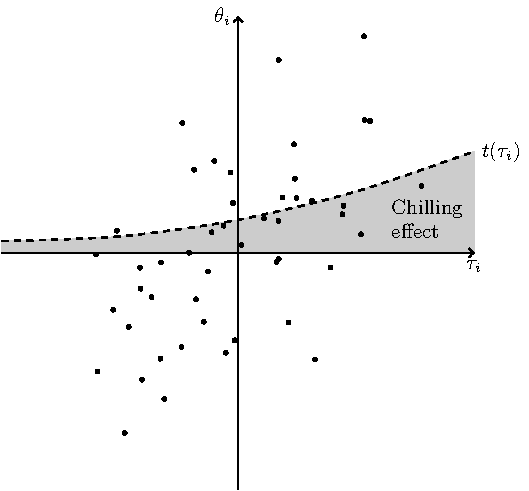
\includegraphics[scale=0.95]{graphchilling.pdf}
\end{frame}

\begin{frame}[label={sec:orgheadline13}]{Welfare results}
\begin{block}{Lemma (Consumer surplus)}
Expected consumer surplus in the information aggregation stage is maximal at the privacy cutoff \(t^p(\tau_i)=0\).
\end{block}
\begin{itemize}
\item welfare includes OP payoff (OP might loose from privacy)
\end{itemize}

\begin{theorem}[Welfare]
Let \(\delta'>0\).

For \(n\) sufficiently large, expected consumer surplus is higher under privacy and OP payoff is the same under privacy and no privacy.

Let the disutility of A be \(-r\delta(\tau_i)\). For \(r\) sufficiently high, consumer surplus is higher under privacy and OP payoff is the same under privacy and no privacy.
\end{theorem}
\end{frame}

\begin{frame}[label={sec:orgheadline14}]{Privacy is redistributive}
\begin{itemize}
\item individuals with \(\theta_i<0\) loose from privacy
\item individuals that are chilled \(\theta_i\in[0, t^{np}(\tau_i)\) gain a bit from privacy
\item individuals with \(\theta_i>t^{np}(\tau_i)\) gain double from privacy (decision, OP interaction)
\end{itemize}
\end{frame}


\begin{frame}[label={sec:orgheadline15}]{Surveillance performs worse than expected}
\begin{itemize}
\item seems as eliminating privacy could give OP huge benefit
\item but: behavior change (chilling) might reduce correlation between \(p_i\) and \(\tau_i\)
\item technical assumption (TA): \(\mathbb{E}[\tau_i|\theta_i=0]\geq 0\) \linebreak (if OP knew \(\theta_i>0\), A would be his best response)
\end{itemize}

\begin{block}{Lemma}
Assume TA. OP's payoff without privacy is lower if individuals use \(t^{np}\) than if they used \(t^p=0\).
\end{block}
\end{frame}

\begin{frame}[label={sec:orgheadline16}]{Surveillance performs worse than expected}
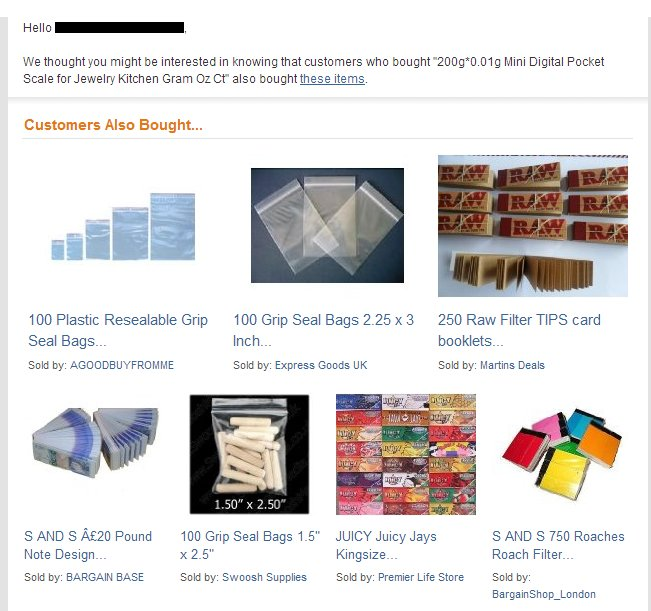
\includegraphics[scale=0.4]{example1}
\end{frame}

\begin{frame}[label={sec:orgheadline17}]{More stuff in the paper I}
\begin{itemize}
\item Extension: privacy as opt in
\begin{itemize}
\item individuals can choose whether to keep \(p_i\) private or not
\item multiple equilibria
\item privacy is not a robust equilibrium: unraveling
\end{itemize}
\item Extension: defensive action
\begin{itemize}
\item Alice can hire a lawyer to help her with the employer
\item \(i\) can take costly defensive action that reduces the disutility of A and lowers the payoff of OP (regardless of his action)
\item equilibria where OP is strictly better off with privacy
\end{itemize}
\end{itemize}
\end{frame}
\begin{frame}[label={sec:orgheadline18}]{More stuff in the paper II}
\begin{itemize}
\item Alternative utility specification: private decision
\begin{itemize}
\item stage 1: no information aggregation, i.e. no externalities from \(p_j\) on \(i\)
\item additional result: privacy is welfare optimal if correlation between \(\theta_i\) and \(\tau_i\) is not too high
\end{itemize}
\item Alternative utility specification: state matching
\begin{itemize}
\item stage 1: payoff of each \(i\) is \(p\theta\) where \(\theta\) is an unknown state and each \(i\) has a noisy signal \(\theta_i\)
\item same results but privacy makes every \(i\) better off as chilling inhibits efficient information aggregation
\end{itemize}
\end{itemize}
\end{frame}
\section{Applications}
\label{sec:orgheadline22}
\begin{frame}[label={sec:orgheadline20}]{Application and discussion: Credit scoring}
repayment probability (\(\tau_{i}\)) is not directly observable
\begin{itemize}
\item Consider two preferences (two different \(\theta_{i}\)) that are predictive of \(\tau_{i}\): education and music taste
\item Low education and a preference for rap music predict low repayment probability.
\item There is a chilling effect in both cases, but in the first we might consider it desirable!?
\item Should the bank be allowed to use data on music taste? (``Equal Credit Opportunity Act'' outlaws ``redlining'' in the US)
\item blacklist vs. whitelist
\end{itemize}

\vspace*{0.6cm}
\begin{footnotesize}
(plausibility: facebook owns patent on making credit scores from its user data)
\end{footnotesize}
\end{frame}

\begin{frame}[label={sec:orgheadline21}]{Application and discussion: Working in committees}
\begin{itemize}
\item committee is debating two policies (e.g. raise interest rates or not)
\item debate and vote can either be in secret or in public
\item correlation between policy preference \(\theta_{i}\) and competence \(\tau_{i}\)
\item members worry about being perceived as incompetent; advocate less radical positions
\item Fed is forced to publish minutes of FOMC meetings since 1993; \linebreak studies show an increase in conformity and a decrease of disagreement with the chairman (Meade and Stasavage 2008)
\item Thomas Hoenig, President of the Kansas City Fed: ``The \emph{tape has had some chilling effect on our discussions}. I see a lot more people reading their statements.''
\end{itemize}
\end{frame}


\section{Conclusion}
\label{sec:orgheadline24}
\begin{frame}[label={sec:orgheadline23}]{Conclusion}
\begin{itemize}
\item we give a simple model to understand privacy from the perspective of information economics
\begin{itemize}
\item no privacy leads to chilling effects
\item privacy can be welfare optimal
\item privacy is redistributive (similar to freedom of speech, Friedman 72)
\end{itemize}
\item the model leads to interesting policy questions
\begin{itemize}
\item blacklist vs. whitelist
\item how open should government be?
\item mandate vs. option of privacy
\item which kind of data should be accessible by who?
\end{itemize}
\item we identify crucial elements to address these questions (correlation, behavior change, threat potential)
\end{itemize}
\end{frame}
\end{document}